\chapter{Introduction}
\label{chapter:intro}
\epigraph{\textit{So kaputt kriegst du mich nie, das schaff ich nur ganz alleine}}{Von Wegen Lisbeth}

\section{Prolog}
\label{sec:prolog}
My time as a student hopefully and finally ends with this work, my thesis.
I started studying physics quite some time ago and honestly doing research for my doctorate feels very different from what university was before.
While there are many things to write here as objective as possible, most of it is still tainted with my style.
Therefore I want to use this prologue as a short but important personal summary.
Working on problems nobody has solved or thought about is hard.
Creativity is an essential skill to perform research.
Doing what everybody does is easy, doing what other people tell you to do is easy.
Finding my very own way to approach problems and designing computational experiments was unbelievable hard work. 
Not only did I do far more things wrong than right, but I also had a naive and idealistic view of science.
But science is done by humans and not by perfectly objective entities\footnote{An AI, as of today, is far away from being an objective entity.}.
Doing research can be fairly disappointing on the one hand or very rewarding on the other.
For me it was mostly the former and while failures or null results are an integral part of science they rarely make into publications.
A situation which at least from my point of view does not improve the quality of research.
It is well known that most of academia's staff is showing symptoms of burnout and are exposed to constant elevated levels of stress~\cite{gewin2021pandemic, bilge2006examining, henny2014prevalence, watts2011burnout, satinsky2021systematic}.
I am just a PhD student, but even I felt guilty during weekends for enjoying the weekend.
Is this a sustainable way to educate and far more important is this a healthy work environment?
One could say, ``well the first three years are bad, but then it gets better``. 
Truth is that the situation of scientists in academia is not optimal, where chain contracts are only one issue.
The requirement of moving to different countries, acquiring funds and publishing research all at the same time is by all means an unhealthy one.

While this may sound depressing, I think it is an opportunity.
An opportunity to make things better, healthier and the first step is to talk openly about the situation.
That is why I choose to add quotes at the start of every chapter.
These quotes are not famous words from important people, they are parts of lyrics from songs.
Songs that highlight that our society is flawed.
Problems such as the requirement that everyone should be perfect out of the box or the constant repression of minorities for example.
I think these lyrics are quite fitting to describe the state I found myself in during being a student and even more so during the writing of this thesis.

\section{Thin Liquid Films}
Thin liquid films appear in multiple forms. 
Many of these forms are not even recognized by us.
Of course, some thin film phenomena will be explained in a more detailed manner throughout this thesis. 
A visual representation of thin film flows can be found in Fig.~\ref{fig:examples_intro}.
\begin{figure}
    \centering
    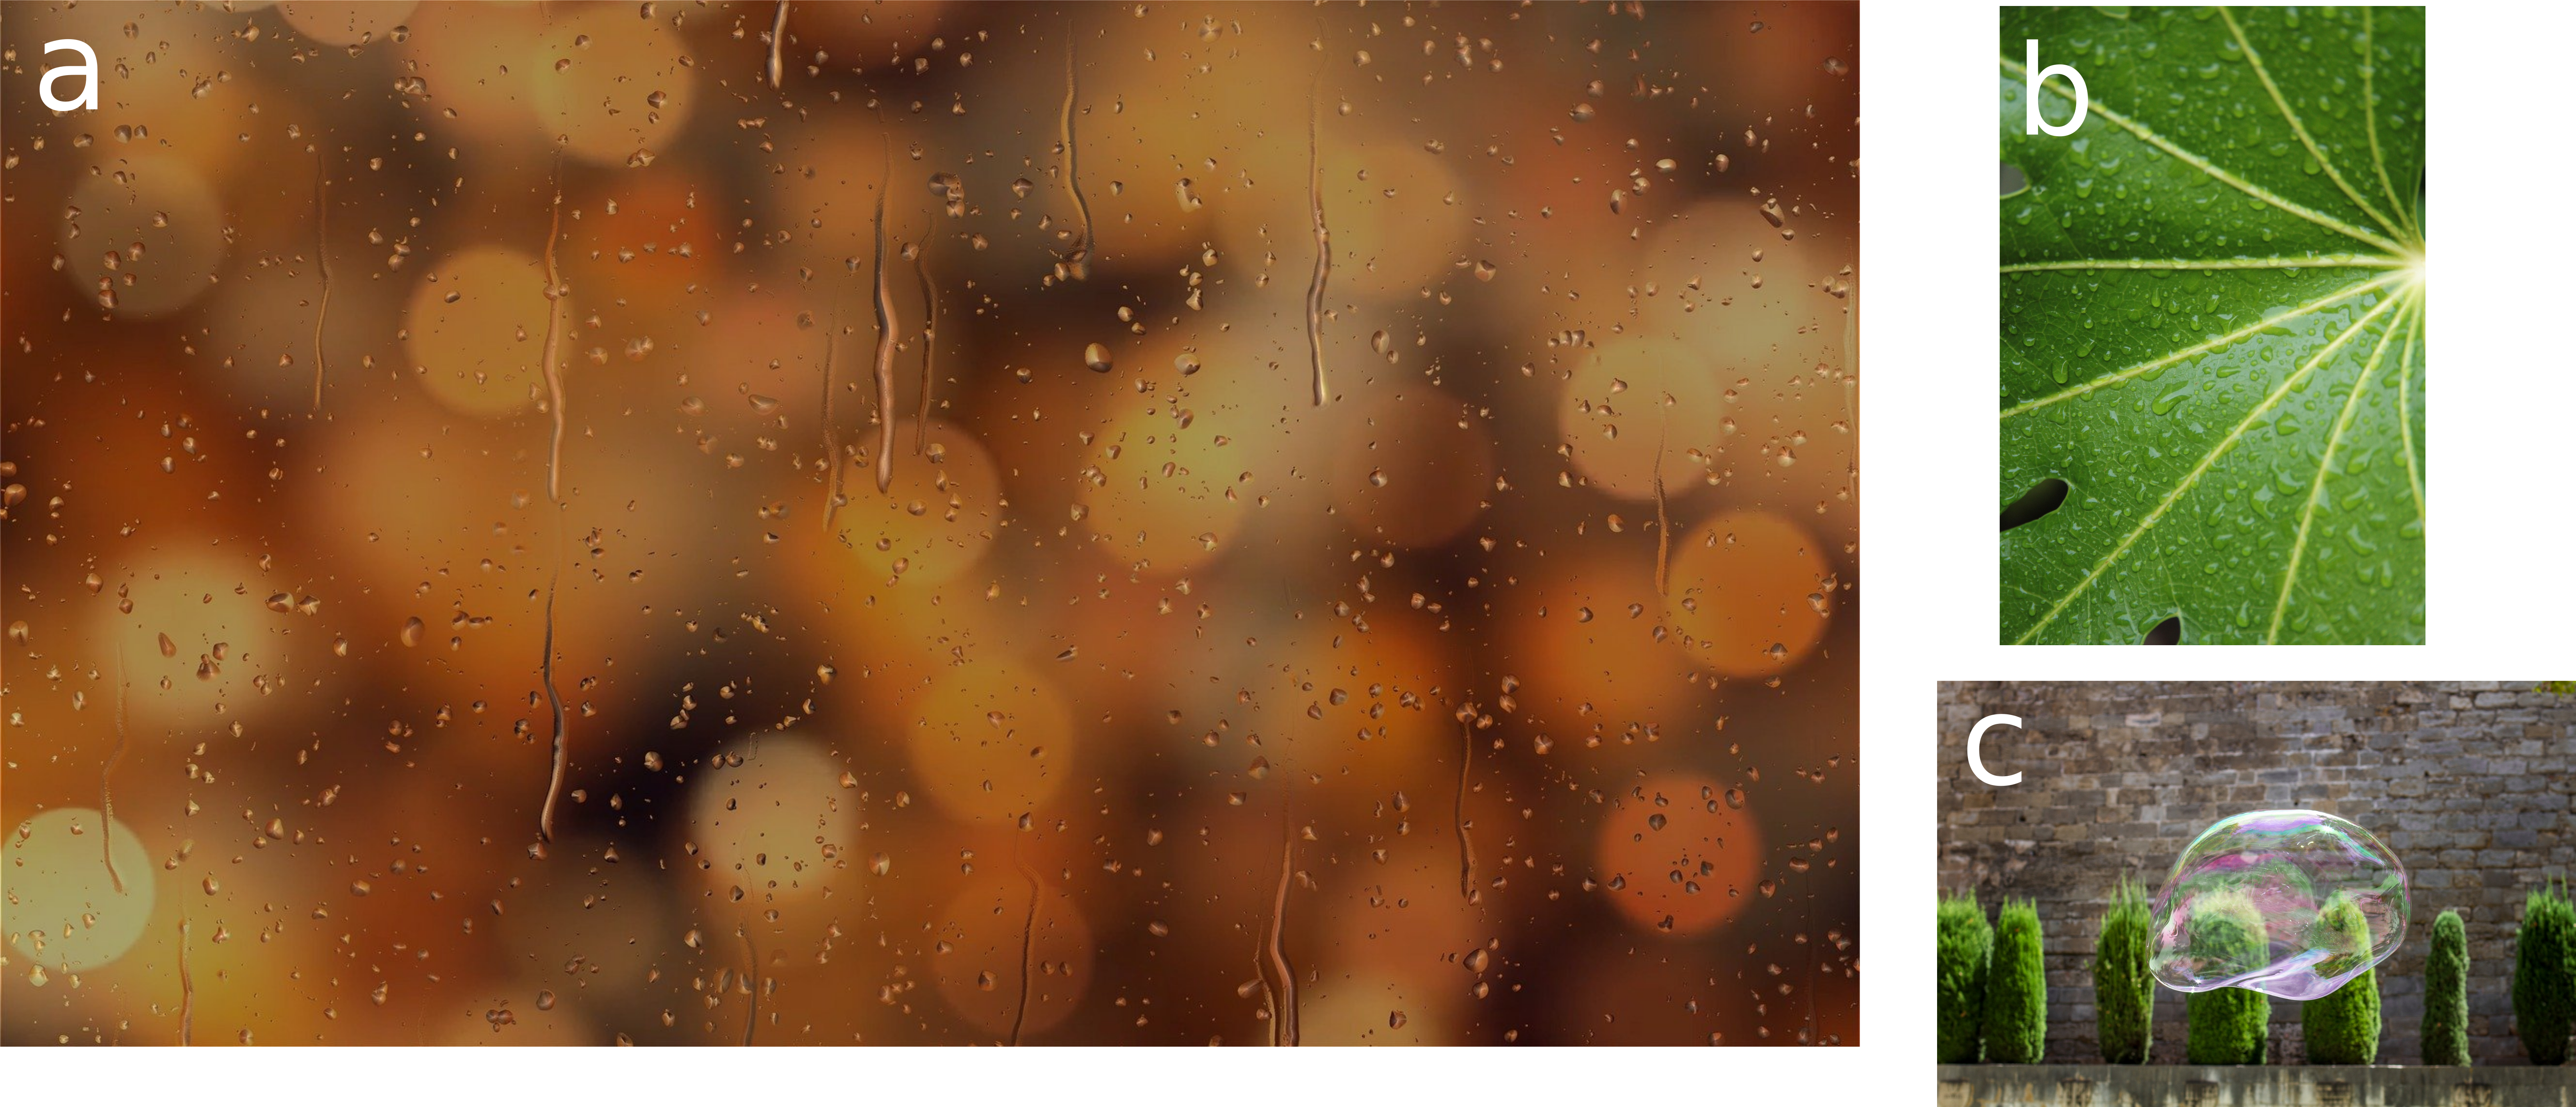
\includegraphics[width=0.95\textwidth]{graphics/Three_tile_intro_smaller.png}
    \caption{Illustrative examples of thin film flows. In (a) rain drops seem to choose random paths running down a window, during their motion they leave behind smaller drops which is called pearling. Tile (b) displays the interaction between water and a plant leaf. Drops are formed quickly and due to the curvature of the leafs surface droplet coalescence is enhanced. Soap bubbles are a prime example of a thin film flow, as shown in (c). A small amount of liquid is enclosed between two gas phases. Inside the film fluid is drained to the bottom of the bubble due to gravity.}
    \label{fig:examples_intro}
\end{figure}

To describe thin film problems however one has to start somewhere.
And the starting point for me and this thesis was to learn about the governing equations of fluid dynamics. 
Those equations are called the Navier-Stokes equations\footnote{strictly speaking the Navier-Stokes equation is a momentum equation, however it is often accompanied with an continuity equation}, and they resemble the dynamics of a fluid constraint due to several symmetries~\cite{Navier, Stokes}, e.g. conservation of mass and momentum.
Solving these equations in a strict mathematical manner, therefore showing existence and smoothness of a solution is an elusive quest. 
Although being around for roughly two centuries this equation is among seven other problems which are considered to be worth a million dollars when solved. 
The collection of these problems is called ``Millenium problems'' and the Navier-Stokes equation poses one of the six unsolved problems.
Nevertheless with the constant innovation in computing techniques and, more so, computing hardware it became more often than not possible to \textit{brute force} an approximate solution for a large class of fluid dynamic problems.
Some examples to be named are the air flow around an airfoil or the catamaran boat structure to reduce drag. 
The main topic of my work however is the dynamics of thin liquids film which admits a crucial simplification to the Navier-Stokes equation. 
Nevertheless it should be noted that theoretical and numerical fluid dynamics (CFD) is by all means a complex but also a vibrant and constantly evolving field.

Generally there are three paths to study the dynamics of thin liquid films.
One can work with the partial differential equations and derive the dynamics from them. 
This is the theoretical approach which uses analytical ansätze and calculus to derive solutions.
On the other hand it is possible to perform experiments with well defined protocols.
Experiments can be set up relatively easy for thin films, one does not need a particle accelerator but often good optics with cameras for high frame rates. 
The time series of images or other control parameters allow, then to derive results from observations.
Both, however theory as well as the experiment have shortcomings. 
Theoretical assumptions can be wrong or the resulting system of equations can be to complex too be solved. 
Experiments often do not allow for the very fine grained control and independent change of different parameters.
The third approach, which is used throughout this thesis lies in between the experiment and a pure theoretical one.
Numerical modelling or computational fluid dynamics allows to approximate the complex partial differential equations while also allowing for fine grained parameter studies.

To study thin films I needed to broaden my understanding of (numerical) modelling. 
What simplifications can I use and are used in common research and how can I introduce these simplifications into my models? 
More so I learned about algorithms and numerical techniques to e.g. test simplifications, especially the Lattice Boltzmann method(LBM)~\cite{doi:10.1146/annurev.fluid.30.1.329, PhysRevE.56.6811, PhysRevE.65.046308, krueger2017}.
The picture of me sitting in front of a monitor, constantly reading research articles and writing code does have little to do with how tangible the field of thin liquid film hydrodynamics can be.
Whenever some liquid advances on a yet dry surface or the distribution of paint on a fresh canvas both can also be looked at from a thin film perspective~\cite{THIELE2014399, RevModPhys.69.931, Edwardse1600183}. 
At some point in our life most of us watched rain drops run down a transparent window~\cite{PhysRevLett.119.204501}, as shown in Fig.~\ref{fig:examples_intro}a. 
The question of why a drop chooses his very own path has a lot to do with the windows surface topology and the three phase contact line (TPC) of the drop~\cite{cassie1944wettability, suzuki2008sliding, doi:10.1021/acs.langmuir.5b02335}. 
Why droplets form at all, e.g.  after a foggy morning can be studied in the framework of the thin film equation as well~\cite{zhang2015inkjet,shi2018fog}.
Although these phenomena happen in many situations their theoretical understanding is far from being complete.
Just to highlight one of the above mentioned situations, the wetting of a dry surface is a highly sophisticated problem.
Using the thin film equation as a mathematical model comes short in explaining the wet-dry transition.
Even worse, to move the liquid on top of a dry surface one would need an infinite amount of energy.
This has to do with boundary conditions and is called the \textit{Huh-Scriven paradox}, which states: ``Not even Herakles could sink a solid if the physical model were entirely valid''~\cite{HUH197185}.
In fact the quote has to be understood in two ways. 
First and foremost, the thin film equation is rather a powerful tool in modelling for a lot of fluid dynamic problems.
Second is the criticism on the rough approximations, i.e. about the \textit{no-slip} boundary condition, which requires a vanishing flow velocity at the substrate.
Of course nature finds a way around and does not use infinite amounts of energy to make a droplet slide. 
In the end the \textit{no-slip} boundary condition is just a model.
Definitely one of the better models, but one that comes short explaining wetting sufficiently well.

I hope that this manuscript will help to understand what kind of problems can be modelled with approaches similar to the thin film equation.
In that sense I want to show how broad the use cases are and where possible extension can lead to.
Having these use cases, both academic as well as industrial, I hope to create an understandable and tangible image of thin film flows. 
Following this short illustrative part will be, of course, the introduction of the mathematical models with their partial differential equations (PDE). 
However this is nothing more than an efficient way of describing the problem.
Strictly speaking mathematics as well as algorithms serve as tools not as the goal of this thesis. 
Therefore I try my best to keep it as simple as possible with analogies and hopefully self explaining figures.

\section{Coating a thin film application}
\label{section:applications}
\begin{figure}
    \centering
    \includegraphics[width=0.75\textwidth]{graphics/41563_2003_Article_BFnmat788_Fig1_HTML.png}
    \caption{Film dewetting of a surface in the spinodial regime.
    Series (a) are experimental measurements with an AFM, while series (b) is generated using a numerical approach with the same parameters taken from~\cite{becker2003complex}.}
    \label{fig:becker_dewetting}
\end{figure}
Applications of the thin film equation are fairly broad as outlined above.
One of the more interesting problems from a scientific point of view is the coating of surfaces.
There are various ways to coat a surface with arbitrary kinds of liquids.
What is common to all of them is the fact that the process heavily relies on the affinity between the to be coated surface and the coating agent~\cite{RevModPhys.81.739}.
If this affinity is too small the coating is unstable and therefore making the film prone to wrinkling~\cite{DASILVASOBRINHO19991204} or eventually even rupture~\cite{RevModPhys.69.931, RevModPhys.81.1131, becker2003complex}, as shown in Fig~\ref{fig:becker_dewetting}.

\begin{figure}
    \centering
    \includegraphics[width=0.75\textwidth]{graphics/Coating_intro.pdf}
    \caption{(a) Schematics of the dip coating process. 
    A substrate is withdrawn from a fluid bath, due capillarity and wetting some liquid adheres to the substrate.
    Most of the liquid however is due to viscous drag not drawn with the substrate.
    A small portion depending on the surface tension and atmospheric pressure is evaporating.
    (b) Schematics of a slot die coating process.
    A die is placed on top of a constantly moving foil.
    Through that die a liquid is pumped onto the moving foil.}
    \label{fig:dip_coating}
\end{figure}
For different object sizes but also for different materials there exists different coating approaches.
One of these approaches is the so called dip coating, as displayed in Fig.~\ref{fig:dip_coating}(a). 
Much like the name suggests the to be coated object is dipped into a reservoir of coating liquid~\cite{scriven_1988, darhuber2000selective, grosso2011exploit}.
While the process itself is straightforward the \textit{art} of dip coating is fairly complex.

From a theoretical point of view this problem has first been addressed by Landau and Levic~\cite{landau1988dragging} as well as Derjaguin~\cite{derjaguin1993thickness}.
Derived in the above work were two limits concerning the dynamics of the film during the extrusion.
In the low extrusion velocity limit, assuming the simple geometry of a plate, one can neglect the contribution due to gravity.
The resulting equation leads to a balance between capillary and viscous forces. 
The film that is drawn with the object is usually very thin and the resulting meniscus between the object and the fluid reservoir is in size proportional to the capillary length.
In fact the thickness of the coating film is roughly given as $h_{\infty} \propto l Ca^{2/3}$, where $l$ is the capillary length and $Ca$ the capillary number.
The capillary number $Ca$ is one among many non-dimensional numbers.
It compares viscous drag with surface tension, whereas the capillary length $l$ is a length scale that separates between gravity and capillary driven dynamics.
This can be understood simply by looking at droplets. 
As long as the volume is small the droplet will form a spherical cap.
If the volume becomes too large, a paddle will form with a distinct difference in shape from a spherical cap, because gravity can no longer be neglected.
In the converse limit of high extrusion velocity the capillary forces become subdominant.
Therefore viscous forces are being balanced with gravity. 
Using the same scaling argument as before the coating thickness can be approximated with $h_{\infty} \propto l Ca^{1/2}$.
Clearly these two regimes show that the extrusion velocity of the coated object has a significant impact, assuming that the surface tension and viscosity are constant parameters.

In case of die or slot die coating the to be coated object is not immersed into a reservoir of coating liquid.
Instead the coated material is usually an elastic foil which moves with constant velocity under a die.
A film is created because the coating fluid is pumped through the die which is placed on top of the foil with some distance $d$.
Similar to the illustration in Fig.~\ref{fig:dip_coating}(b), a film is drawn due to balance between capillary and viscous forces.
The thickness of the resulting film however does not depend on gravity in this case.
Ruschak showed that similar to the low extrusion velocity limit of the dip coating problem the film thickness after die coating can be approximated using $h_{\infty} = d~Ca^{2/3}$~\cite{RUSCHAK19761057}.

These two examples highlight an important behaviour.
The solutions consists of some variable, here the capillary number, that scales with a well defined exponent, e.g. $2/3$ and $1/2$.
These results can be addressed as dimensional analysis, a rather fancy word for getting the exponent correct because in the end the height or thickness needs to be of the dimension of a length.
They often support so-called self similar behaviour, thus upon rescaling results with a quantity it can be possible to derive a single master curve for all data. 

\section{Literature Overview}
\label{section:literature}
\begin{figure}
    \centering
    \includegraphics[width=0.85\textwidth]{graphics/reynolds_slip_bearing.pdf}
    \caption{A drawing from Osborn Reynolds on slipper bearing lubrication.
    The four figures are taken from ref.~\cite{ReynoldsLubr} and cropped together in a single image.
    Displayed is the load balance between the lubricant and the solid body on top.}
    \label{fig:reynolds_work}
\end{figure}
Theory concerning lubrication is a little bit younger than the Navier-Stokes equation~\cite{Navier, Stokes}. 
Osborn Reynolds was the first to work on the problem of slipper bearing, as shown in Fig.~\ref{fig:reynolds_work}.
The idea of the slipper bearing is to reduce the wear of moving mechanical components due a lubrication fluid, in Reynolds case that fluid was olive oil~\cite{ReynoldsLubr}.
Within this work Reynolds developed what is called today the lubrication approximation.
Instead of solving the problem in all it's glory, Reynolds derived that due to constraints the problem can be simplified. 
The first constraint is the fact that the film's thickness $H$ is much smaller than it's lateral extension $L$ and therefore $\varepsilon = H/L \ll 1$. 
Besides this ratio the liquids inertia can be neglected as the acceleration of the fluid is slow.
Variations along the liquid interface are smooth thus the gradient $|\partial h/\partial x_i| \ll 1$ for both lateral dimensions.
This clean and novel deduction dates back already to the year 1886 and will be further discussed in Chap.~\ref{chapter:theory}.

Since the 19$^{\text{th}}$ century the theory of lubrication had gain much attention and got extended to account for more complex problems.
Over time it became it clear that problems such as wetting and capillarity can be studied within this framework~\cite{RevModPhys.57.827, RevModPhys.69.931, RevModPhys.81.1131}.
To this end the term thin film equation was introduced, which is nothing more than the functional form that the lubrication approximation yields. 
Wetting for example does strongly depend on the intermolecular forces. 
The DLVO potential made it possible to account for these forces~\cite{derjaguin1941acta, verwey1947theory}. 
DLVO is an acronym from the name of the four scientists Derjaguin, Landau, Verwey and Overbeek who developed this theory. 
Initially this potential was used to understand the stability of colloidal suspensions, however for thin film theory it offers a quantification for the disjoining pressure~\cite{RevModPhys.69.931, Peschka9275, moulton_lega_2013, PhysRevE.63.011208}.
Pierre-Gilles de Gennes, who was awarded with the Nobel Prize in physics in 1991 for his work on soft matter physics and his students were ones of the first who understood that ``\textit{dirty}'' soft matter physics can help in understanding thin film problems~\cite{RevModPhys.57.827,doi:10.1021/la0116342,de2013capillarity}.

Of course, by end of the 20$^{\text{th}}$ century there were already some yet unexplained experimental findings associated to the thin film equation, e.g. the spectrum of capillary waves~\cite{doi:10.1021/ja01014a015}.
While the spectrum was quickly connected with thermal fluctuations it took theory some time to catch up.
From a theoretical point of view one has to account for the stochastic nature of thermal fluctuations.
Entry point for this problem is not the Navier-Stokes equation but the Landau-Lifshitz Navier-Stokes (LLNS) equation~\cite{Landau1987Fluid}.
The stochastic thin film equation is then, again, derived from the Landau-Lifshitz Navier-Stokes by integration along the vertical dimension.
This step however poses a hard problem, because the stochastic stress tensor in principle depends on the vertical dimension.
Grün and coworkers found an elegant way to circumvent the problem with a single multiplicative gaussian term~\cite{Grun2006, Mecke_2005, PhysRevLett.99.114503, PhysRevE.102.053105, PhysRevE.100.023108, PhysRevE.92.061002}, the idea will be revisited in Chap.~\ref{chapter:second_paper}.
Around the same time Davidovitch et al. came up with a similar form for the stochastic thin film equation, studying the spreading of a droplet~\cite{PhysRevLett.95.244505}.
The addition of a gaussian noise term made it therefore possible to reproduce the observed capillary wave spectrum and explain the difference in spreading behaviour.
A further impact of this term was the reduction of rupture times for spinodal dewetting thin films~\cite{Grun2006, PhysRevLett.99.114503}.
Becker et al. pointed out that the classical thin film equation comes short in prediction of the experimentally measured rupture times~\cite{becker2003complex}.
In fact the rupture time is overestimated by the classical thin film equation, adding however thermal fluctuations do decrease the rupture times~\cite{Duran_Olivencia2019, shah_van_steijn_kleijn_kreutzer_2019}.

Additions of complex dynamics on top of the partial differential equation that defines the thin film problems is not limited to thermal fluctuations.
On the one hand it is possible to add degrees of freedom to the fluid. 
For example one can study the effect of non-Newtonian shear behaviour~\cite{zhang2005non, myers2005application}. 
Or inclusion of arbitrary concentration fields to induce Marangoni-like flows~\cite{sultan_boudaoud_amar_2005, C5SM01603G, PhysRevLett.93.247803}.
Even the previous example of thermal fluctuations~\cite{Grun2006, Mecke_2005, PhysRevLett.95.244505, PhysRevE.104.034801}
On the other hand the substrate can be e.g. chemically or topographically patterned.
A modified substrate can lead to a very different understanding of wetting behaviour as shown in refs.~\cite{cassie1944wettability, WHYMAN2008355}.
In 2019 the Deutsche Forschungsgemeinschaft (DFG) funded the priority program 2171: ``\textit{Dynamic wetting of flexible, adaptive and switchable surfaces}''.
The goal of this program is to enlarge the understanding concerning the dynamics of thin liquid film on complex substrates.
Therefore substrates with internal degrees of freedom.
For example substrates with a grafted polymer brushes or special treatment to generate a self-cleaning super hydrophobic surface similar to the lotus leaf effect~\cite{doi:10.1021/acs.langmuir.0c03226, thiele2020gradient, doi:10.1021/acsnano.9b08211}.
Picking up the example of the lotus leaf, it is not necessary that the substrate is stiff.
In fact most organic structures are not as stiff as a silica substrate (or the glass of a window), therefore wetting of soft materials is as well considered in this priority program~\cite{doi:10.1146/annurev-fluid-010719-060147, https://doi.org/10.1002/nme.6567, chen2011short}.
More so with special surface treatment it is possible to control the substrates surface chemistry~\cite{xin2010reversibly, WANG200718}.
These stimuli respondent substrates are collected under the umbrella of the term \textit{switchable substrates}.
Allowing for the dynamic control of the substrates wettability with e.g. light sources~\cite{doi:10.1126/science.288.5471.1624, doi:10.1246/bcsj.20180076}.
\begin{figure}
    \centering
    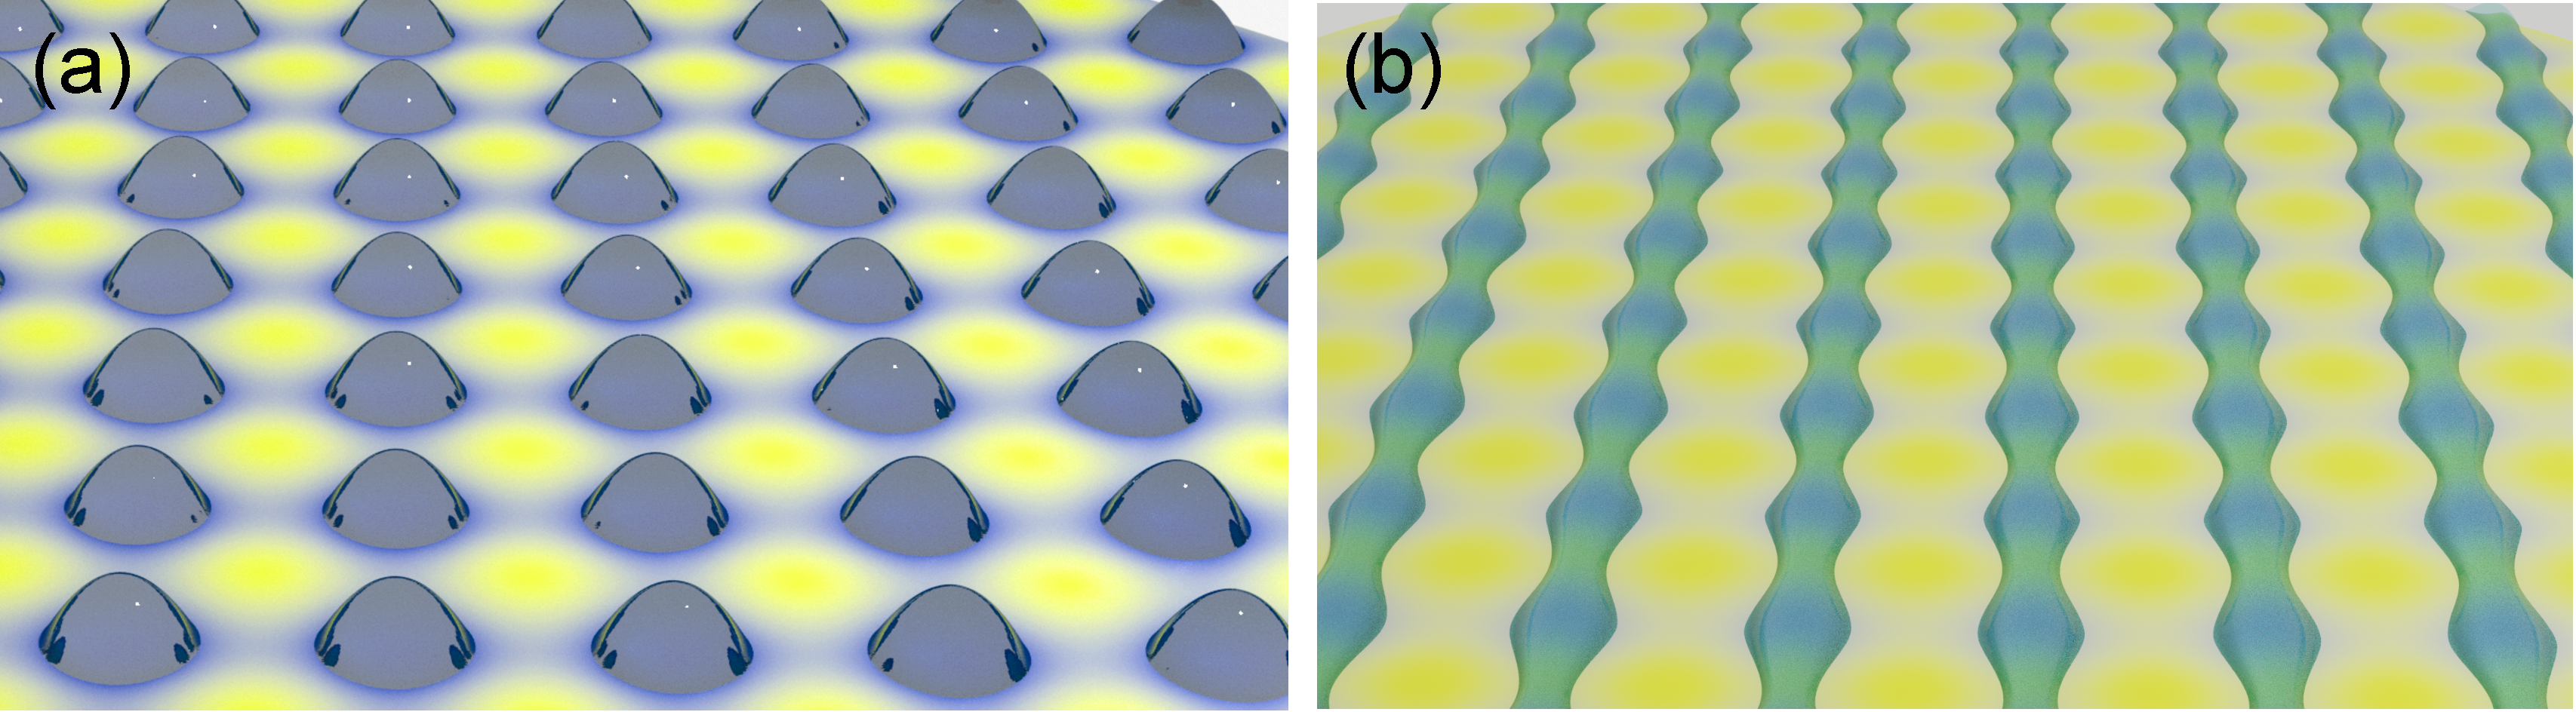
\includegraphics[width=0.88\textwidth]{graphics/no_v_lig.pdf}
    \caption{(a) Equilibrium state of a dewetting thin film on a patterned substrate, i.e. droplets inside of the contact angle minima. 
    The color corresponds to the contact angle. 
    Yellow shows a high and blue a low contact angle, ranging from 10$^{\circ}$ to 30$^{\circ}$. 
    (b) Similar to the left panel a dewetting thin film on a ``switchable'' substrate. 
    Due to the function that controls the contact angle field liquid rivulets are formed.}
    \label{fig:morph_transition}
\end{figure}
This opens up a new avenue for microfluidic devices.
In Chap.~\ref{chapter:third_paper} we discuss the influence a switchable wettability can have on the dewetting of a thin film.
In fact the switching can induce morphological transitions as depict in Fig.~\ref{fig:morph_transition}. 

\section{Scientific Software}
\label{section:statement_software}
The way thin liquid films are studied in this thesis is by using analytical models for computer simulations.
Therefore I build and use software to run numerical experiments.
Software is a central part of our society.
The interaction with an operating system, the quick information distribution over emails and the web calls via e.g. Zoom have become standard rituals of our work life (because due to Corona we had to change the way we usually interact with people).
Most of the time these applications work.
When they do not work it induces stress\footnote{Just the outage of a computational infrastructure for running simulations lead repeatedly to elevated levels of stress.}, because we rely on them and yet have barely any control.

While it is easy to say that ``\textit{software should work}'' it is hard to guarantee.
The complexity of writing good source code and working applications is at least comparable to that of a scientific problem.
In fact, good software has become so complex that the workforce of a huge margin of employees of a company can be used up on a problem as ``simple'' as a search engine.
To make it possible to work in cooperation at this scale it is necessary to use so called \textit{best practises} and \textit{style guides}~\cite{sommerville2004software}.
Such style guides could for example define how to add and test new functions.

Scientific software is often seen as a secondary or by-product of research and sadly often threaded that way.
In contrast to the peer review process for scientific findings and publications, software that generated scientific results is rarely tested by reviewers.  
While there are high standards to industrial software, e.g. Ansys Fluent~\cite{matsson2020introduction}, these standards are quite low for the average scientifically developed source code.
This however is fairly troubling due two reasons.

Software or source code is prone to bugs because it is a creative process.
One approach to overcome the issues of bugs is the so called test driven development (TDD) approach~\cite{beck2003test}.
The simple idea is that, whenever a function is written it is accompanied with one or more test cases.
Using this principle creates a testing suite that (hopefully) ensures that functionality is not broken if changes to the source code are made.
For mature software projects, e.g. OpenFOAM~\cite{jasak2007openfoam, jasak2009openfoam, chen2014openfoam}, these suits can be even integrated into the continuous development/continuous integration (CD/CI) step and therefore be automated.
Often however when a student starts a new software project, functionality or performance is the main point of interest.
During the development step tests and even more important documentation are left aside.
Ultimately this does not only open the gate for various bugs but to some extent it also renders the software useless for other researchers.
Needless to say, my very own implementation of the solver, see Chap.~\ref{chapter:fourth_paper}, generated correct results due to the cancellation of two bugs.
Defining a test suite from the beginning of the project would have spared me valuable time and effort.

On the other hand, research became more than ever dependent on computational resources.
Clearly the main topic of this thesis, computational fluid dynamics is a compute heavy subdomain of fluid dynamics. 
However recent advances in artificial intelligence show a rising trend to their applicability for industrial and scientific problems~\cite{acemoglu20198, doi:10.1080/14685248.2020.1797059}
This advances comes at a price, leaving aside the discussion if artificial intelligence is of value at all.
One of the main pillars that generates trust in scientific results is their reproducibility.
Independent of the number of trials a stone, when flung up in the air, will fall to the ground following a well defined path\footnote{Given the stone is not flung with earth's escape velocity, $v\approx 11.2$km/s}.
Generating huge amounts of data without labels and explanation makes it by definition impossible to verify any given finding or result from that experiment.
Mislabeling data is not something new, it always happened from time to time with e.g. laboratory journals.
However exa-scaling computing pushes this problem to new severity.
Now or never is the time to install protocols. 
Guides on how to deal with scientific software such that data can be reproduced or even more important reused.
While this may not be of interest for most readers, to me it is an essential point.
That said, Chapter~\ref{chapter:fourth_paper} describes the software developed and used for this thesis. 
One can find the open source software repository that hosts the code, tests and documentation.
Upon pull or merge requests an automated testing suite performs tests to ensure no bugs break necessary functionality.
Furthermore by definition of version control it is possible to reproduce all results generated with that software.

\section{Outline}
\label{section:outline}
Following this short introduction are the key concepts of this thesis.
Starting with the next Chapter~\ref{chapter:theory} a detailed explanation of the theoretical ideas is presented.
Thus the starting point will be the equations of motion of a fluid, the Navier-Stokes equation.
Using real world observations and strong assumptions the Navier-Stokes equations can be reduced to the Saint-Venant or shallow water equations~\cite{saint1871theorie, williamson1992standard}.
Astonishingly similar arguments play a critical role in the derivation of the thin film equation.
However these two kinds of systems describe different physical phenomena.
Still, as will be shown, this a direct consequence of \textit{long-scale}, \textit{long-wave}  phenomena~\cite{RevModPhys.69.931}.
Chapter~\ref{chapter:theory} will then end with a short section of differences and intersections between these two theories.

In Chapter~\ref{chapter:method} numerical frameworks for solving differential equations are presented.
Starting with a short overview of different methods to be used to solve the thin film problem.
Therefore introducing the concept of discrete differentiation, spectral methods via fast Fourier transformation and molecular dynamics (MD).
Showing that different length and time scales can be a pitfall for either of these methods.
In between the macro (classical Navier-Stokes solvers) and micro (molecular dynamics and density functional theory) scale is the lattice Boltzmann method, a so-called meso-scale approach.
The underlying differential equation that is solved is the Boltzmann equation and not the Navier-Stokes or the equation of motion for each molecule.
However as will be shown the Navier-Stokes equation can be approximated using the lattice Boltzmann method~\cite{Enskog, Chapman, doi:10.1146/annurev.fluid.30.1.329, krueger2017}.  
Not only is it possible to approximate the Navier-Stokes but also the shallow water equations, of course with a different set of constraints~\cite{Salmon:1999:0022-2402:503, zhou2004lattice, van2010study, PhysRevE.65.036309}.

Following that argumentation is the submitted manuscript for the \textit{Journal of Open Source Software}. 
Highlighting the implementation and development of the lattice Boltzmann solver called \textbf{Swalbe} (\textbf{s}hallow \textbf{wa}ter \textbf{l}attice \textbf{B}oltzmann solv\textbf{e}r) in Chapter~\ref{chapter:fourth_paper}.
Key aspects are the automated continuous integration (CI) with a test suite and web-hosted documentation, as motivated in Sec.~\ref{section:statement_software}.
The Julia package allows for either fast iterative model development in two dimensions or large scale simulations in three dimensions with GPU acceleration.
Therefore having a playground for prototyping and testing which is fast and easy to use.
But also a framework for large three dimensional simulations with minor to no code changes.

Use case and a derivation of the model can be found in Chapter~\ref{chapter:first_paper}.
Showing the mandatory assumptions which make it possible to approximate the thin film equation with the shallow water lattice Boltzmann model.
With some emphasis on the numerical implementation of e.g. the computation of gradients and the Laplacian in agreement with ref~\cite{doi:10.1137/S1064827599357188, THAMPI20131}. 
After the derivation, numerical experiments are displayed to validate the model. 
Among those are the Rayleigh-Taylor instability, e.g. a film hanging from a plate. 
Spreading dynamics is tested against the Cox-Voinov and Tanner's laws. 
The linear relation between Bond and Capillary number is validated with the sliding of a droplet.
Closing the chapter with a discussion on the performance of the algorithm and applicability for accelerated computing.

In the next chapter, Chap.~\ref{chapter:second_paper}, a functional extension to the lattice Boltzmann model is shown.
Instead of approximating the deterministic thin film equation the stochastic thin film equation (STF) is the topic of interest in this chapter.
Thermal fluctuations are often neglected in simulations while their existence in the experiment can not be denied.
For nanometric thin films fluctuations can accelerate the time scales of instabilities. 
Interestingly the time scales of these instabilities and resulting film ruptures are in fact contact angle dependent.
Depending however on the substrates properties (patterning), it is still likely that fluctuations are only subdominant.

Dynamics during dewetting can either be generated due to forces, as shown in Chapter~\ref{chapter:first_paper}-\ref{chapter:second_paper} or it can be induced due to time dependent potentials. 
Giving the recent interest in dynamics of simple liquids on complex substrates in the Priority Programme 2171, thus dynamic wetting of flexible, adaptive and switchable surfaces, Chapters~\ref{chapter:fourth_paper} is dedicated to question: ``What happens during dewetting with a spatio-temporal evolving wettability gradient?''
To study this question a series of three dimensional simulations are performed with varying spatial as well as temporal evolution of the wettability.
On the one hand the wettability dynamics has a small but measurable stabilising effect on the spinodal dewetting thin film.
Leading to a net increase in rupture times if the dynamic wetting is switched on.
On the other hand after the rupture of the film a clear morphological transition is observable.
Having only a static wettability gradient results in stationary droplets in regions of high wettability.
Making the wettability gradient dynamic, can lead to metastable rivulet states.
These rivulets can be explained using a simple model that balances the capillary with the wettability wave velocity, introducing a cutoff parameter ($\Gamma > 1$) for which rivulets are to be observed.

In the last Chap.~\ref{chapter:conclusion} a summary and conclusion of the work collected in this thesis is given.
Summarizing the scientific results that have been achieved during the duration of the PhD.
Because this work can be seen as an ''\textit{exploratory}''\footnote{A statement that Prof. S. Karpitschka made after my talk in the MPI-DCF seminar.} work, some outlook is presented with possible extensions as well as further dynamical variables to study more complex thin film flows. 